\documentclass[a4paper,12pt]{report}
\usepackage[utf8]{inputenc}
\usepackage[francais]{babel}
\usepackage{graphicx}
\usepackage{fancyhdr}
\usepackage[absolute]{textpos}
\usepackage[svgnames]{xcolor}
\usepackage{colortbl}
\usepackage{lastpage}
\usepackage{url}
\usepackage[colorlinks,citecolor=DeepPink4,linkcolor=DarkRed,urlcolor=DarkBlue]{hyperref}
\usepackage{geometry}
\usepackage{tikz}
\usepackage{titlesec}
\usepackage{datetime}
\usepackage{lipsum}
\usepackage{enumerate}
\usetikzlibrary{matrix}

\newcommand{\doctitle}{CDC3}
\newcommand{\doclongtitle}{Cahier des Charges 3}

\title{\doctitle{} Vigilate}
\author{Soules Kévin, Mercier Daniel, Budowski Prune, Harscoat Morgane, Poncet Manuel, Keller Flavien}
\date{\today}

\definecolor{myBlue}{RGB}{23,54,93}
\newdateformat{slashdate}{\twodigit{\THEDAY}/\twodigit{\THEMONTH}/\THEYEAR}

\titleformat{\section}[block]{\bfseries}{\thesection.}{1em}{}
\titleformat{\subsection}[block]{\hspace{2em}}{\thesubsection}{1em}{}
\titleformat{\subsubsection}[block]{\hspace{3em}}{\thesubsubsection}{1em}{}
  
\geometry{
  a4paper,
  left=20mm,
  right=20mm,
}

\setlength{\unitlength}{1mm}
\addtolength{\headheight}{1.5\baselineskip}
\renewcommand{\headrulewidth}{0.0pt}
\renewcommand{\footrulewidth}{0.4pt}


\fancypagestyle{eip}{
  \fancyhf{}
  \fancyhead[L] {
    \includegraphics[width=3cm]{../../logos/logo_eip.png}
  }
  \fancyhead[R] {
    \colorbox{myBlue}{
      \textcolor{white}{
        \Large \textbf{[2017][Vigilate][\doctitle{}]}
      }
    }
  }
  \renewcommand{\headrulewidth}{0pt}
  \fancyfoot[L]{
    \textcolor{gray}{
      \{EPITECH.\}
    }
  }
  \fancyfoot[C] {Vigilate \textbar{} \today{}}
  \fancyfoot[R]{
    \ifnum\value{page}>0
    \thepage/\pageref{LastPage}
    \fi
  }
}

\makeatletter
\let\ps@plain\ps@eip
\makeatother

\pagestyle{eip}


\begin{document}
\date{\slashdate\today}
\setcounter{page}{-4}

% --- (1) Page de garde ---

\thispagestyle{empty}
\vspace*{\stretch{2}}
\begin{center}
  \textcolor{myBlue}{\Huge \textbf{EIP Vigilate}}\linebreak
  \vspace*{\stretch{1}}
  \textcolor{gray}{\textit{\Large \doclongtitle{} (\doctitle{})}}\linebreak
  \vspace*{\stretch{1}}
  {\today}
\end{center}
\vspace*{\stretch{1}}
\newpage

% --- (2) Résumé ---

\vspace*{\stretch{1}}
\begin{flushleft}
  \textcolor{myBlue}{\textit{\large \textbf{Résumé du document}}}\linebreak
\end{flushleft}
Le cahier des charges commence par un bref rappel de notre EIP, Vigilate, un outil de sécurité informatique qui permet de se tenir informé des dernières vulnérabilités publiques rapidement sur tous les programmes que l’utilisateur souhaite vérifier. On mettra en avant les contraintes fonctionnelles et les exigences non-fonctionnelles comme le fait que notre projet doit être sécurisé, ou alors la réactivité de notre outil. Notre projet est réalisé par 6 personnes. Le document présente d’une part la structure du projet : un site web, le back-end, une machine virtuelle et un scanneur de programme et d’autre part, les différentes fonctionnalités du projet à partir d’un document UML (connexion de l’utilisateur, possibilité de modifier ses préférences : programmes à surveiller, style d’alerte souhaité...). Nous présentons dans la partie 6 l’organisation prévue : 2 personnes sur le site web, 2 sur le back-end, 1 sur la machine virtuelle et 1 sur le scanneur de programme. Ainsi que la méthodologie utilisée, basée sur la méthode Agile (Scrum). Pour ce faire, nous devons construire un produit backlog avant de commencer à développer le projet, puis organiser un nombre de sprints adéquat, d’une durée relativement courte (principe de la méthode agile) mais qui permettront d’avoir un projet fonctionnel à chaque fin de sprint avec chaque tâche décrite dans un backlog de sprint. Nous présenterons également l’environnement et les outils utilisés (github pour héberger nos documents...). Nous avons réalisé un template de mise en page pour toute notre documentation avec Latex. Nous avons choisi de respecter la norme Python Pep8 pour le développement. Dans une dernière partie, nous proposerons une description des tests, utilisés pendant le développement notamment grâce à l’outil Travis et les tests une fois l’outil terminé.\\
\vspace*{\stretch{1}}
\newpage

% --- (3) Cartouche + révisions ---

\begin{flushleft}
  \vspace*{\stretch{1}}
  \textcolor{myBlue}{\textit{\large \textbf{Description du document}}} 
  \bigbreak
  \begin{tabular}{|>{\columncolor[RGB]{220,220,220}\color{Navy}\bfseries}l|p{12cm}|}
\hline
Titre & [2017][Vigilate][\doctitle{}] \\
\hline
Date & 31/01/2015 \\
\hline
Auteur & Kévin SOULES \\
\hline
Responsable & Kévin SOULES\\
\hline
Email & vigilate\_2017@labeip.epitech.eu\\
\hline
Sujet & \doclongtitle{}\\
\hline
Mots clés & \doctitle{}, sécurité, vulnérabilités\\
\hline
Version du modèle & 1.1\\
\hline
\end{tabular}


  \vspace*{\stretch{2}}
  \bigbreak
  \bigbreak
  \textcolor{myBlue}{\textit{\large \textbf{Tableau des révisions}}}
  \bigbreak
  \small
\begin{tabular}{|p{1.5cm}|l|p{2.5cm}|p{7.8cm}|l|}
  \hline
 
   \rowcolor{Gainsboro}Date  & Auteur & Section(s) & Commentaires \\
  \hline
24/01/15 & Kévin Soules &  & Création du documents\\
  \hline
27/01/15 & Kévin Soules & Chapitre 1 et 2.1 & Recherche de liste de solutions. Rédaction du texte d'un premier concurrent. Remplissage des rappels.\\
\hline
28/01/15 & Prune Budowski & Chapitre 1 & Amélioration des rappels \\
\hline
29/01/15 & Prune Budowski & Chapitre 3.3.2 & Rédaction de la partie ``Ce qui ne sera pas couvert''\\
\hline
29/01/15 & Daniel Mercier & Chapitre 2.2 & Rédaction du texte du deuxième concurrent.\\
\hline
29/01/15 & Kévin Soules & Chapitre 2.3 & Rédaction du texte du troisième concurrent. \\
\hline
30/01/15 & Morgane Harscoat & Chapitre 2.4 & Début de rédaction du texte du quatrième concurrent. \\
\hline
30/01/15 & Kévin Soules & Chapitre 2.5 & Rédaction du texte du cinquième concurrent.\\
\hline
31/01/15 & Kévin Soules & Conclusion, Glossaire & Matrice de préférence.Rédaction d'un glossaire. \\
\hline
31/01/15 & Prune Budowski & Résumé, Conclusion, Chapitre 3.1 & Rédaction du résumé. SWOT. Rédaction de la partie ``Ce que vous apportez''.  
  \\
\hline
31/01/15 & Daniel Mercier & Toutes & Corrections. \\
31/01/15 & Prune Budowski & & Mise en page. \\
31/01/15 & Kévin Soules & & Mise en page.
\\
  \hline
\end{tabular}
\normalsize

  \vspace*{\stretch{1}}
\end{flushleft}

% --- (4) Tables des matières ---

\tableofcontents

% --- (5) Rappel eip ---

\textcolor{myBlue}{\chapter{Rappel de l'EIP}}
\setcounter{page}{1}
\section{Qu'est-ce qu’un EIP et Epitech}
Epitech,  école de l'innovation et de l'expertise informatique propose un cursus en 5 années, basé sur une pédagogie par projet (à réaliser seul ou en groupe). L'un de ces projets, l’EIP (Epitech Innovating Project), réalisé par groupes de 6 à 15 étudiants, démarre au cours de la 3\ieme année et se déroule sur 2 ans et demi. Ce  projet doit être particulièrement innovant, car son objectif est d’être commercialisable à la fin de la 5\ieme année d’Epitech.

\section{Sujet de votre EIP}
Le but de Vigilate est d’avertir les utilisateurs des services obsolètes ou potentiellement vulnérables affectant en particulier leur infrastructure (sites web, réseau d'entreprises, logiciels), dans le but de les informer des risques techniques encourus et des éventuelles mises à jour ou corrections à appliquer.
Cela sans effectuer de scan de vulnérabilité.
Nous proposons cependant un outil de scan de programme qui envoie la liste sur notre plateforme web.

\section{Glossaire}
\noindent
\vskip 0.1cm
\textbf{- C -}\\
\vskip 0.1cm
\textit{CVE (Common Vulnerabilities and Exposures)}: dictionnaire d'informations publiques relatives aux vulnérabilités informatiques. Par métonymie, on emploie souvent le terme CVE à la place de CVE ID (ou identifiant CVE), qui lui désigne le numéro qui renvoie à la fiche descriptive complète de cette vulnérabilité. Exemple: CVE-2013-4343.\\
\textit{CSIRT (Computer Security Incident Response Team)}: équipe chargée d'assurer la sécurité d'une entreprise.\\
\textit{CERT (Computer Emergency Response Team)}: marque déposée représentant les CSIRT certifiés.\\
\vskip 0.1cm
\textbf{- F -}\\
\vskip 0.1cm
\textit{Fingerprint}: déduction de la version d'un programme/système d'exploitation en fonction de la façon dont il répond à nos requêtes sur le réseau.\\
\textit{Fork}: création d'un nouveau programme en utilisant le code source du premier.\\
\vskip 0.1cm
\textbf{- G -}\\
\vskip 0.1cm
\textit{GPL (General Public License)}: licence dédiée aux logiciels libres.\\
\vskip 0.1cm
\textbf{- P -}\\
\vskip 0.1cm
\textit{Patch}: un correctif qui corrige un bug ou une vulnérabilité dans un programme.\\
\vskip 0.1cm
\textbf{- S -}\\
\vskip 0.1cm
\textit{SCADA (Supervisory Control and Data Acquisition)}: système de télégestion à grande échelle utilisé dans l'industrie.\\



% This is where we add the \input for all the other pages.

\textcolor{myBlue}{\chapter{Contraintes}}
\section{Contraintes fonctionnelles}
\begin{itemize}
\item Portabilité\\
La portabilité sera la principale contrainte fonctionnelle à laquelle la réalisation du projet devra se plier. La machine virtuelle devra être conçue de façon à pouvoir être utilisable sur les systèmes d'exploitation les plus répandus, il en va de même pour le site web, devant impérativement prendre en charge une grande majorités de navigateurs, à jour ou non, afin que son fonctionnement ne soit pas altéré selon la configuration de l’utilisateur.
\end{itemize}

\section{Exigences non fonctionnelles}
\begin{itemize}
\item Simplicité de l'interface\\
Dans un souci de simplicité d'utilisation, il faudra que l'interface utilisateur de notre système soit intuitive et à la portée de tous, de façon à favoriser la prise en main de cette solution par un utilisateur lambda, n'ayant aucune compétence avancée en informatique.\\
Différents types d'alertes pourront être envoyés au client, une alerte détaillée concernant la vulnérabilité, ses détails techniques et ses caractéristiques, pouvant être destinée à l'équipe informatique du client, et une alerte plus concise pouvant par exemple être destinée à un responsable.

\item Réactivité\\
Afin d'optimiser l'efficacité de notre solution, la réactivité est l'un des points clés à respecter.\\
Dans le but d'informer les utilisateurs des vulnérabilités les concernant dans les plus brefs délais, nous nous devrons de concevoir et maintenir un système réactif au niveau la récupération et la transmission des données, cela permettant au client de faire corriger les vulnérabilités de son système au plus vite.\\

\item Concevoir un système et une plateforme sécurisés\\
Le but de notre solution étant de favoriser la sûreté des services utilisés par nos clients, avoir un produit et une infrastructure stables fait également partie des points clés à respecter. Il sera donc impératif de sécuriser correctement le site, les différents services que nous utilisons et par conséquent le stockage de nos données, afin d'éviter toutes fuites de données relatives à un client, à son système informatique, ou à notre propre infrastructure. Enfin, le système en machine virtuelle destiné à être installé chez le client devra être développé de façon à être imperméable à toute forme d'attaque actuellement prévisible, il va de soi qu'après sa fonction principale de détection et d'alerte, la priorité de ce système concerne le fait qu'il ne puisse, ou le moins possible, être lui-même compromis par une attaque informatique.
  
\end{itemize}

\textcolor{myBlue}{\chapter{Description des différentes parties du programme à réaliser}}
\section{Structure générale}
Vigilate est une solution composé de 3 programmes différents :\\
\begin{itemize}
\item Un site web\\
\item Un scanner\\
\item Un backend\\
\end{itemize}
Vigilate pourra optionnellement être distribué sur une vm.\\
\section{Le site web}
Le site web servira à la personnalisation des alertes. On pourra choisir quels programmes suivre. On pourra aussi choisir un niveau de criticité minimum par programme  pour être prévenu. Le site permettra aussi de choisir le ou les moyens par lesquels on veut être prévenu lors de la découverte d’une vulnérabilité (mail, sms ou notifications sur le site). Le site web enverra ces données au backend via l’api pour qu’il mette à jour la base de donnée.\\
Le site web utilisera django côté serveur, la communication avec l’api se feras donc en python. Cotés client il utiliseras angularJS afin de mieux interagir avec l'utilisateur\\

\section{Le scanner de programme}
Le scanner de programmes est là par soucis de simplicité d’utilisation, ce sera un programme en python (donc portable) qui récupérera la liste des programmes installés et les enverra au backend via l’api pour mettre à jour la base de donnée. Le scanner pourra être lancé manuellement ou planifié pour s’exécuter régulièrement (par exemple une fois par semaine).\\

\section{Le Backend}
Le backend sera le coeur de vigilate. C’est un programme qui récupérera les cve dès leurs sortie via le flux rss du site cve.mitre.org. Une fois récupérées il les stockera dans la base de données et regardera si un des clients utilise ce programme, si c’est le cas il vérifiera ensuite si la version est vulnérable. Puis il ira voir si le niveau de criticité est égale ou supérieur à celui précisé par le client via le site web, si c’est le cas il préviendra le client par tous les moyens que celui-ci aura choisi.\\
Le backend recevra aussi  les informations du scanneur et les stockera dans une base de donnée.\\
Le backend hébergera aussi l’api de vigilate, cette api permettra au backend de communiquer avec le scanner et le site web, elle récupérera leur requêtes et fera les modifications nécessaires dans la base de données. L’api permettra de modifier la liste de programmes installés et leurs versions ainsi que de changer les préférences (niveau de criticité et moyen de contact).\\
Il y aura aussi une API publique. Cette API sera utilisable par client qui souhaite intégrer Vigilate à leur solution. On peut par exemple imaginer un hébergeur qui propose le service vigilate à ses clients afin qu’il puissent monitorer la sécurité des programmes qu’ils utilisent.\\
Le backend seras lui aussi codé en python, les API public et interne seront de type REST. Ce qui permettra une utilisation simple et clair avec angularjs.\\


\section{La vm}
Pour finir Vigilate offrira optionnellement une vm.\\
Les serveurs de Vigilate contiendront la liste des programmes de chaque utilisateur. Ces informations peuvent être sensibles si elles appartiennent à des entreprises ayant besoin d’un grand niveau de sécurité. Vigilate en mode VM répond à ce problème.
\\
Ce sera machine virtuelle prête à fonctionner qui contiendra le site web et le backend de vigilate. Un système de mises à jour permettra à la vm d’avoir les composants de vigilate constamment à jours sans avoir à la réinstaller. La vm restera connecté à notre API de façon chiffrée et sécurisée, afin de récupérer les nouvelles vulnérabilités qui sont publiées. C’est la VM qui se charge de comparer l’information avec ses données locales pour envoyer ou non les alertes de sécurité.
\\
Vigilate en mode VM permet aux entreprises critiques de garder en local les informations sensibles de sécurité de leur infrastructure. Aucune information sortira du réseau, en effet la VM utilise seulement un flux réseau descendant pour les mises à jour.


\section{Cas d’utilisation}
\begin{figure}[!h]
  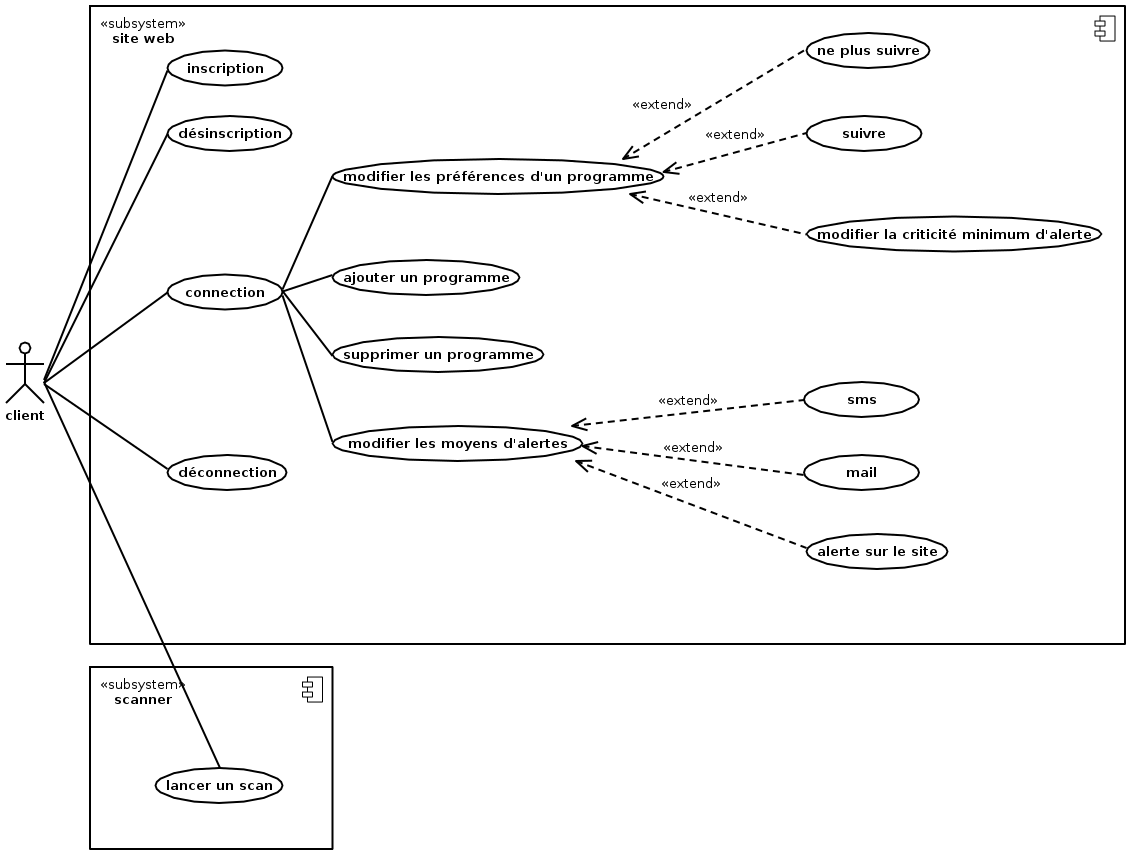
\includegraphics[width=18cm]{uml1.png}
\end{figure}
\begin{figure}[!h]
  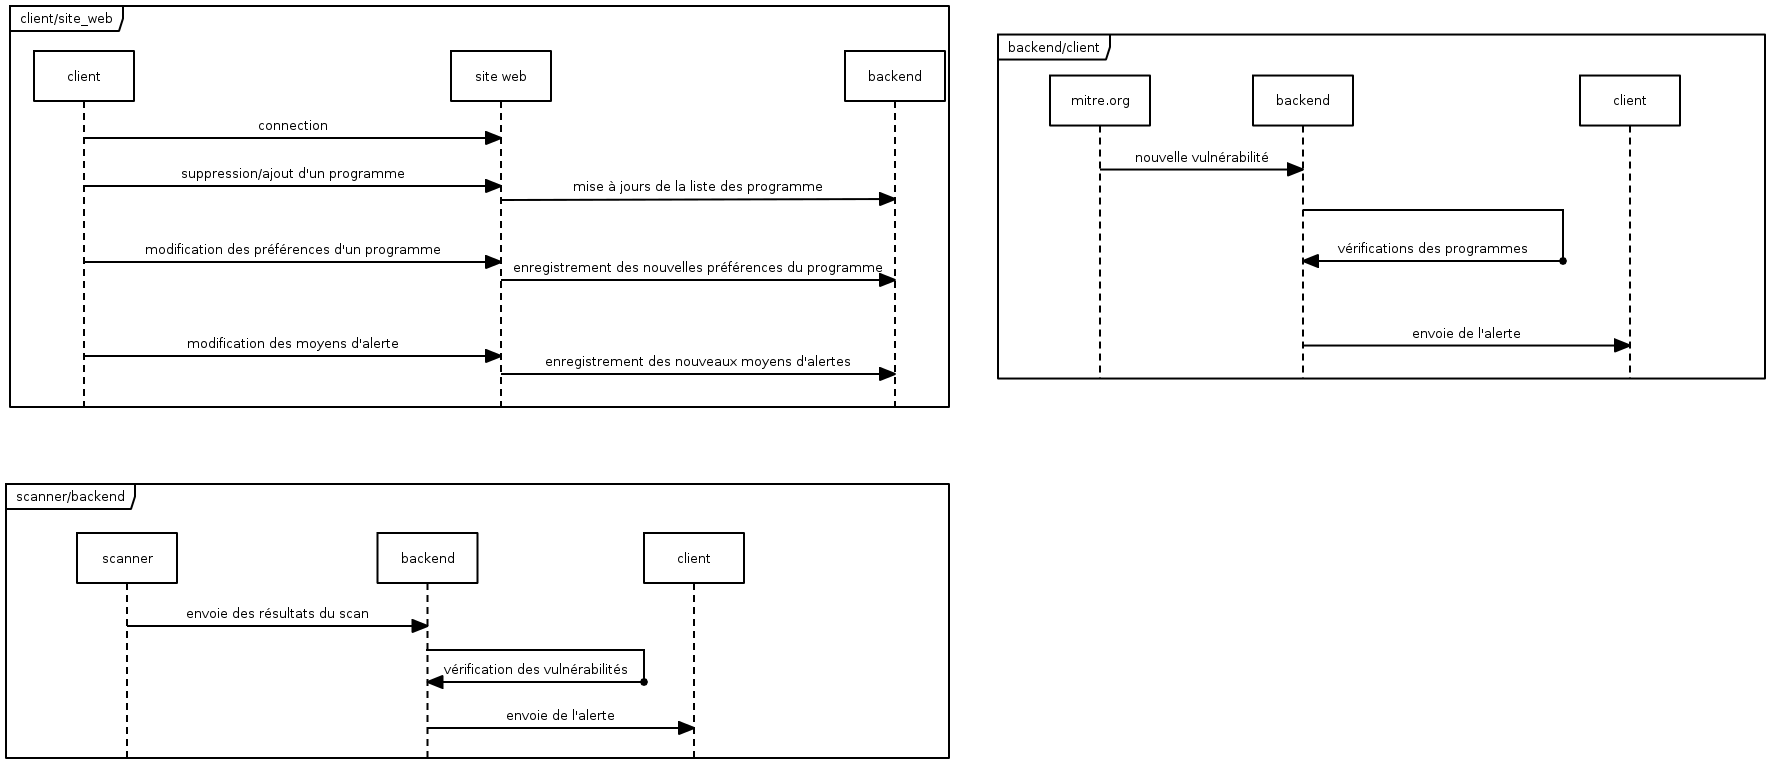
\includegraphics[width=18cm]{uml2.png}
\end{figure}


\textcolor{myBlue}{\chapter{Présentation de l’environnement de réalisation}}
\section{Environnement de réalisation}
Notre environnement sera composé des outils suivants:\\
- github, une plateforme de gestion et d'hébergement de projet. Système de gestion de version, Système d’issue.\\
- Travis-ci, un outil permettant de réaliser des tests d’intégration continue sur un projet informatique. Avant de valider un commit, cette plateforme compile le projet et lance les tests unitaires.\\
- Python, le langage de programmation qui sera utilisé afin de réaliser les différentes tâches.\\
- LaTeX, langage permettant de mettre en forme un document texte. Cet outil sera utilisé pour la documentation.\\
- pep8, la norme de programmation que l’on respectera pour python.\\

\section{Composants existants}
Afin de récupérer les informations sur les nouvelles vulnérabilités, nous nous baserons sur un outil qui liste les dernières CVE.\\
Elles sont listées sous la forme de flux RSS, nous suivrons ce flux pour rester informer des derniers ajouts.\\
Cette source d’information est donc la source d’information principale que nous utiliserons.\\

\section{Gestion de la sécurité}
Nous somme un outil de sécurité, donc on se doit  d’avoir une infrastructure exempte de vulnérabilité. Il ne faut en aucun cas qu’une personne puisse accéder aux informations d’un autre compte.\\

\section{Points sensibles}
Le flux rss que l’on utilisera pour récupérer nos données est un point essentiel de notre solution. Si cette source disparaît, nous devrons trouver un autre moyen pour lister les derrières vulnérabilités. Une solution alternative étant de suivre les mailing list de sécurité et automatiquement détecter les ajout de CVE.\\

\textcolor{myBlue}{\chapter{Description des tests}}
\section{Tests pendant la phase de développement}
\begin{itemize}
\item Utilisation de l'outil Travis CI fourni avec GitHub afin d'assurer une intégration continue du projet.\\
\end{itemize}
Travis permet d'automatiser une batterie de tests à chaque contribution au projet et permet par la même de rejeter la contribution si elle ne valide pas la série de tests pré-programmés.\\
De cette façon, l'intégration continue grâce à Travis Ci nous permet de s'assurer que chaque modification ne produit pas de régression au sein du développement du projet.\\

 
Travis nous permet donc d'automatiser les tests de régression et d'avoir l'état précis de l'avancement du projet.\\

\section{Tests avant la sortie final}
\begin{itemize}
\item Test d'intrusion complet (white box) garantissant la sécurité de l'ensemble de la solution. Cette analyse en profondeur de la sécurité de notre solution nous permet de garantir la fiabilité et la stabilité de notre projet lorsque celui-ci est confrontée à des attaques diverses et variées. C'est une étape non négligeable dans le développement d'un projet, surtout lorsque le thème abordé est en rapport avec la sécurité applicative.\\
\item Test complet de l'interface utilisateur. Cette étape finale de test est obligatoire dans le sens ou elle nous permet de bien assurer le contrôle qualité de notre produit et évite tout désagrément pour l'utilisateur final.\\
\end{itemize}

\textcolor{myBlue}{\chapter{Organisation projet}}
\section{Méthode de travail}
\begin{itemize}
\item Réunion internes hebdomadaire : Ces réunions nous permettront de nous tenir informés de l’avancement de chacun malgré le décalage horaire et la distance géographique. Durant ces réunions nous parlerons du travail effectué durant la dernière semaine, évoqueront les difficultés que nous avons pu rencontrer afin de nous entraider, cela nous permettra également de donner notre avis sur le travail de chaque membre du groupe et de maintenir une cohésion et une bonne dynamique de travail. Ces réunions nous serviront aussi à préparer les suivis mensuels avec le Lab EIP.\\
\item Méthode Scrum (agile) : Méthodologie qui consiste à créer un product backlog avant le développement en définissant toutes les fonctionnalités du projet avec un niveau de priorité, de fonctionner avec un système de sprints c’est à dire avec des phases de développement assez courtes pour avoir un projet fonctionnel, en suivant un sprint backlog (un liste de tâches précise définit avant chaque sprint). Outil utilisé: redmine.\\
\end{itemize}
\section{Outils de travail}
\begin{itemize}
\item Git : grâce à Git nous pourrons constater de l’avancement de chaque membre et consulter le travail des autres de manière simplifiée. Nous pouvons ainsi nous entraider et accéder à la dernière version du projet sans démarche spécifique de notre part, tout est automatiquement mis à jour pour tous les membre sur le répertoire.\\
\item Hangout : nous utilisons une discussion Hangout afin de pouvoir communiquer facilement en interne malgré le décalage horaire entre les membres. Nous utilisons également la fonctionnalité Appel de Hangout pour nos réunions hebdomadaires.\\
\item Travis : à chaque commit sur github, Travis exécute une batterie de tests afin de vérifier que le projet est toujours fonctionnel et que des bugs n’ont pas été ajoutés.\\
\item Redmine : cet outil de gestion de projet nous permettra de bien appliquer les méthodes agiles, faciliter notre travail durant le développement de Vigilate ainsi que de respecter nos jalons.\\
\end{itemize}
\section{Planning}
\begin{itemize}
\item 09/15 : Développement de Vigilate\\
\item 01/16 : Communication passive (page facebook, site vitrine, twitter, newsletter...)\\
\item 09/16 : Bêta test interne du projet\\
\item 09/16 : Lancement d’actions de communication\\
\item 12/16 : Produit fini\\
\item 01/17 : Tests finaux\\
\item 01/17 : Soutenances finales\\
\end{itemize}


Semaine type de travail :\\
\begin{itemize}
\item 1 journée dédiée au travail sur l’EIP\\
\item 1 réunion interne\\
\end{itemize}

\section{Répartition du travail}
La réalisation de Vigilate sera découpée en “grandes parties” qui seront assignées à chaque membre du groupe de la manière suivante. (Bien sûr il n’est pas exclu qu’un membre intervienne sur la partie de quelqu’un d’autre de manière ponctuelle en cas de besoin.)\\
\begin{itemize}
\item Site web (2 personnes)\\
\item Programme de scan (1 personne)\\
\item Backend / API (2 personnes)\\
\item Machine virtuelle (1 personne)\\
\end{itemize}

\textcolor{myBlue}{\chapter{Conclusion}}
\section{Matrice de préférence}
\thispagestyle{plain}

Dans cette matrice de préférence, nous comparons plusieurs points importants: la réactivité à une nouvelle menace, la simplicité d’utilisation de l’outil, la cible et enfin la pertinence de l’information qui est remontée.\\
\footnotesize
\bigbreak
\noindent
\begin{tabular}{|p{2.2cm}|>{\raggedright}p{2.8cm}|>{\raggedright}p{3.2cm}|p{2cm}|p{4.9cm}|}
  \hline
  \rowcolor{Gainsboro}Projet & Réactivité & Simplicité & Cible & Pertinence de l'information \\
\hline

  Nessus & Plutôt longue. Réactivité éditeur + temps de scan & Les scans classiques sont simplistes à utiliser mais la personnalisation de ceux-ci est plus compliqué & Entreprises. & Bonne. Seules les vulnérabilités trouvées sont remontées. \\
\hline

  Shalvik Protect & Réactivité égale à celle des éditeurs de programmes. & Très simple il scan et installe les patchs tout seul. & Entreprises. & Bonne. Elle concerne seulement les programmes installés sur la machine. \\
\hline

  CERT/CSIRT & Très bonne. L’équipe est prête à répondre en cas d’urgence. & Très simple pour l’entreprise, ce n'est pas elle qui s’en occupe. & Entreprises, organisations. & Bonne. Elle est adaptée à la cible.\\
\hline

  Cisco Security Manager & Bonne, dès qu’un évènement interne est détecté. & Difficile. Nécessite une connaissance des technologies réseaux. & Entreprises, organisations & Bonne, elle concerne des évènements internes.\\
\hline

  CERT-XMCO & Bonne. Alerte dès qu’un bulletin est publié. & Assez simple. & Entreprises, organisations. & Mauvaise. Tous les bulletins sont affichés, et le filtrage ne se fait pas forcément très bien. \\
\hline

  Vigilate & Très bonne. Dès qu’une vulnérabilité est rendue publique. & Très simple. Ergonomique. & Entreprises, organisations, revendeurs, webmasters, particuliers & Très bonne. Seule l’information qui concerne l’utilisateur est remontée. \\
\hline
\end{tabular}
\normalsize  

\section{SWOT}
L'analyse SWOT est un outil de stratégie permettant de déterminer les options stratégiques envisageables au niveau du domaine d'activité stratégique.\\

\centering
\colorlet{helpful}{lime!70}
\colorlet{harmful}{red!30}
\colorlet{internal}{yellow!20}
\colorlet{external}{cyan!30}
\colorlet{S}{helpful!60!internal}
\colorlet{W}{harmful!50!internal}
\colorlet{O}{helpful!50!external}
\colorlet{T}{harmful!50!external}

\newcommand{\texta}{Positive\\ \tiny (pour atteindre l'objectif)\par}
\newcommand{\textb}{Négative\\ \tiny (pour atteindre l'objectif)\par}
\newcommand{\textcn}{Origine interne\\ \tiny (organisationnelle)\par}
\newcommand{\textdn}{Origine Externe\\ \tiny (environnement)\par}

\newcommand{\back}[1]{\fontsize{60}{70}\selectfont #1}

\begin{tikzpicture}[
  any/.style={minimum width=4cm,minimum height=4cm,%
    text width=3cm,align=center,outer sep=0pt},
  header/.style={any,minimum height=1cm,fill=black!10},
  leftcol/.style={header,rotate=90},
  mycolor/.style={fill=#1, text=#1!75!black}
  ]

  \matrix (SWOT) [matrix of nodes,nodes={any,anchor=center},%
  column sep=-\pgflinewidth,%
  row sep=-\pgflinewidth,%
  row 1/.style={nodes=header},%
  column 1/.style={nodes=leftcol},
  inner sep=0pt]
  {
    &|[fill=helpful]| {\texta} & |[fill=harmful]| {\textb} \\
    |[fill=internal]| {\textcn} & |[mycolor=S]| \back{S} & |[mycolor=W]| \back{W} \\
    |[fill=external]| {\textdn} & |[mycolor=O]| \back{O} & |[mycolor=T]| \back{T} \\
  };

  \node[any, anchor=center] at (SWOT-2-2) {$\bullet$ Informations pertinentes\\ $\bullet$ Personnalisation\\ $\bullet$ Rapidité d'information};
  \node[any, anchor=center] at (SWOT-2-3) {$\bullet$ Pas de scanner de vulnérabilité};
  \node[any, anchor=center] at (SWOT-3-2) {$\bullet$ Besoin de plus de sécurité};
  \node[any, anchor=center] at (SWOT-3-3) {$\bullet$ Beaucoup d'outils existent déjà};

  \end{tikzpicture}


\textcolor{myBlue}{\chapter{Annexes}}
\noindent
pep8: \url{https://www.python.org/dev/peps/pep-0008/} \newline
travis-ci: \url{https://travis-ci.org/} \newline
redmine: \url{http://www.redmine.org/} \newline

\end{document}